\documentclass[letter paper, 11pt]{article}
\usepackage{geometry}
\usepackage{babel}
\linespread{1.3}
\geometry{
	left=15mm,
	right=15mm,
	top=15mm,
	bottom=15mm,
}
\usepackage{amsmath,amssymb,amsthm,amsfonts}
\usepackage{lmodern}
\usepackage[T1]{fontenc}
\usepackage{titlesec}
\usepackage{titling}
\usepackage{verbatim}
\usepackage{float}
\usepackage{enumerate}
\usepackage{enumitem}
\usepackage{amsthm}
\usepackage{titlesec}
\usepackage{multicol, listings}
\usepackage{graphicx}
\usepackage{algorithmic}
\usepackage{algorithm}


\begin{document}
	
	
	\title{%
		Review of Collaborative Filtering in Recommender System \\
		\large Final Project Report of CS 6241}
	
	\author{Wentao Guo}
	
	\date{}
	
	\maketitle
	
	
	\section*{Abstract}		
	
	\section*{Keyword}
	\begin{center}
	SVD, SVD++, Recommender System, Collaborative Filtering
	\end{center}

	
	\section{Background} 
	\paragraph{}
	Developed in 1990s, the recommender system (RS) has been applied in e-commence, music apps, job portal, social networking and more \cite{netflix}. The recommender system collects information on users' behaviors explicitly (users' ratings on items) and implicitly (users' mouse movements, attention on one page, etc.) and makes prediction on users' preferences. For example, Netflix applies a five-star ratings to help users find their favorite movies and maintain their subscriptions \cite{gower}, and Amazon selects products based on the predicted users' favors to gain profits. 
	
	
	In October 2006, Netflix launched a competition for which they rewarded the team that can beat Netflix's Cinematch system by at least 10\% Root Mean Squared Error \cite{gower}. This competition arouse great attention in collaborative filtering field as the dataset covered 100 million ratings for 500, 000 anonymous customers on 17, 000 movies, which was greater than previous public dataset in the orders of magnitude \cite{MFinRS}. The final grand prize was given to "Bellkor's Pragmatic Chaos" team in 2009 \cite{gower} \cite{koren}. 
	
	
	In this competition, matrix factorization approaches raised people's attention as the top teams in this competition frequently applying it to beat Bayes or probabilistic approaches \cite{korenFactorization}. Singular Value Decomposition as the classical latent semantic indexing approach in information retrieval was found as a great fit for spanning customers data with low dimensions and often adapted to various variants as regularized SVD, SVD++, iterative SVD, and more \cite{gower} \cite{SVD++performance} \cite{contextual} \cite{korenFactorization}. 
		
	% some intro to CF
	
	
	\section{SVD-Based CF Methods}
	\subsection{Intro to SVD}
		SVD, as a common dimension reduction tool, originally used in information retrieval to identify latent semantic factor (as Latent Semantic Indexing), can represent the user-item interactions in a low dimensional space \cite{MFinRS} \cite{ApplySVD}. SVD approximates a matrix $A \in \mathbb{R}^{m \times n}$ in a form as 
	\begin{equation}
		A = U \Sigma V^T
	\end{equation}
	Suppose the rank of $A$ is $r$, there are three main properties in SVD\cite{ApplySVD} \cite{gower}:
	\begin{itemize}
		\item 
		The initial $r$ singular values of diagonal matrix $\Sigma$ holds that $\forall i \in [1, r]\,\sigma_i > 0$ and $\sigma_1 \geq \sigma_2 \geq ... \geq \sigma_r$.
		
		\item 
		The first $r$ columns of orthogonal matrix $U$ are eigenvectors of $A\,A^T$ and span the column space of $A$.
		
		\item
		The first $r$ columns of orthogonal matrix $V$ are eigenvectors of $A^T\,A$ and span the row space of $A$.
	\end{itemize}
	
	People usually takes the best rank-$k$ approximation of matrix $A$ as 
	\begin{equation} \label{trun-SVD}
		A_k = U_k \Sigma_k V_k^T
	\end{equation}
	
	with $U_k \in \mathbb{R}^{m \times k}, \ \Sigma_k \in \mathbb{R}^{k \times k}, \ V_k \in \mathbb{R}^{k \times n}$.
	
	\subsection{Standard SVD-Based Neighborhood Approach of Collaborative Filtering}	
	We will take a rating matrix $R$ with users $u_1, u_2, ... u_i$ in the row and items $i_1, i_2, ... i_j$ in the column, and the entry $R_{ij}$ is the estimated interest of user $u_i$ on item $i_j$. \cite{MFinRS} \cite{CF-IterPCA} \cite{ApplySVD}.
	
	Notice that matrix $R$ is often sparse and require some prepossessing. A common prepossessing approach is to take the row averages to replace all of the missing values in the matrix $R$ and normalize $R$ by subtracting row averages \cite{ApplySVD} \cite{CF-IterPCA}.
	
	We then compute $U_k \Sigma_k V_k^T$ as equation \ref{trun-SVD}, and form two matrix products: $U_k \sqrt{\Sigma_k^T}$ and $\sqrt{\Sigma_k} V_k^T$.
	
	There are some variants regarding the computation of predicted rating \cite{ApplySVD} \cite{SVD-performance}. For example, Manolis et al. \cite{SVD-performance} provided a formula for SVD-CF prediction rating for user $u$ on item $i$ as:
	
	\begin{equation}
		\hat{r}_{ui} = \bar{r_u} + U_k \sqrt{\Sigma_k^T [u]} \sqrt{\Sigma_k} V_k^T (i)
	\end{equation}
	
	Another variant is based on PCA, with the previous steps identical except that we need to replace and subtract column average $\bar{c_j}$ for prepossessing $R$. In addition, prediction score for user $u$ on item $i$ will be
	
	\begin{equation}
		\hat{r}_{ui} = \bar{r_i} + U_k \sqrt{\Sigma_k^T [u]} \sqrt{\Sigma_k} V_k^T (i)
	\end{equation}

	Some researchers incorporate the reduced matrix $R_{\text{red}} = U_k \Sigma_k V_k^T$ into the calculation of similarity measure to predict the new user or item's score based on the existing clusters. These approaches are usually categorized to user-based collaborative filtering or item-based collaborative filtering depending on the subject of similarity measure.
	
	
	Pearson correlation and adjusted cosine similarity are common similarity measures in literature\cite{CF}\cite{ApplySVD} \cite{new-sim} \cite{sim-CF} \cite{CF-sign}:
	\begin{itemize}
		\item Pearson correlation
		
		$\mathcal{I}_{uv}$ means common item rated by both user $u$ and user $v$. $\bar{r_u}$ means average rating of user $u$ on the shared item set.
		\begin{equation}
			\text{sim} = \frac{\sum_{i \in \mathcal{I}_{uv}}(r_{ui} - \bar{r_u})(r_{vi} - \bar{r_v})}{\sqrt{\sum_{i \in \mathcal{I}_{uv}}(r_{ui} - \bar{r_u})^2(r_{vi} - \bar{r_v})^2}}
		\end{equation}
		
		\item Adjusted cosine similarity
		
		$\bar{r_u}$ means average rating of user $u$ on the entire item set.
		\begin{equation}
			\text{sim} = \frac{\sum_{i}(r_{ui} - \bar{r_u})(r_{vi} - \bar{r_v})}{\sqrt{\sum_{i}(r_{ui} - \bar{r_u})^2(r_{vi} - \bar{r_v})^2}}
		\end{equation}
	
	\end{itemize}


	Pearson-correlation looks really similar to adjusted cosine similarity except that adjusted cosine similarity is calculated over the entire set of rated vectors while person correlation is calculated over co-rated vector \cite{sim}. For the missing value case, a typical approach is to set it as zero \cite{new-sim}.

	In item-based collaborative filtering, after we calculate similarity measure, we normally select nearest $l$ neighbors and then make the prediction (or compute prediction rating). The first algorithm proposed by Vozalis and Margaritis \cite{ApplySVD} provides a formula as
	
	\begin{equation}
		\hat{r_{ui}} = \dfrac{\sum_{j = 1}^{l} \text{sim}_{ij} * (R_{\text{red}_{uj}} + \bar{r_u})}{\sum_{j=1}^{l} |\text{sim}_{ij}|}
	\end{equation}

	Variants on prediction rating formula exist, but this is one classical approach of item-based collaborative filtering. The process of user-based collaborative filtering is similar to item-based collaborative filtering except the implementation of SVD on $R$ and prediction rating is different. 
	
	If we formulate a framework neighborhood-based collaborative filtering (including user-based and item-based) based on previous steps, we will obtain what Bokde et al. purpose \cite{MF-Model-Survey}\footnote{The prediction rating process can be combined with or separated from recommendation in real practices.}:
	
	\begin{enumerate}
		\item Prepossessing:
		build a user-item matrix and perform dimensional reduction
		
		\item Similarity Evaluation:
		formulate the neighborhood with similarity metrics
		
		\item Prediction Rating Process \& Recommendation:
		calculate the correlation and finally provide a recommendation
	\end{enumerate}
	
	\subsection{Standard SVD-Based Latent Factor Approach of Collaborative Filtering} 
	The previous framework more applies to neighborhood approach. Some researchers are also interested in the framework of "latent semantic model". 
	
	\subsubsection{User-item Interaction in Latent Factor Space}
	Matrix factorization models represents the user-item interaction in a latent joint space \cite{MFinRS}. Each item $i$ is associated with a vector $q_i \in \mathbb{R}^f$ and user $u$ is associated with a vector $p_u \in \mathbb{R}^f$. The rationale behind such representation is: item $i$ will possess some unknown factors in a measure, positive or negative, stored in entries of $q_i$, and user will have different favors toward these factors, and such interest is represented as entries in $p_u$. Therefore, we can take inner product to get an approximate of the user $u$'s rating on item $i$ as \cite{MFinRS} 
	\begin{equation}
		\hat{r}_{ui} = q_i^T  p_u 
	\end{equation}
	
	The latent factor model tries to minimize the prediction error in some metrics. Conventional evaluation metrics includes root mean squared error (RMSE) and mean absolute error (MAE). Researchers usually minimize a function $\mathcal{L}$ to obtain prediction. (Stochastic) Gradient descent will be applied if the problem is convex, or if nonconvex requires other efforts to gain the global optimal solution such as Zheng et al. show \cite{RSVD}.
	
	
	Conventional SVD suffers from an incomplete (or even sparse) rating matrix. Researchers often resort to imputation to fill in the matrix, or through regularized least squared model as \cite{MFinRS}.
	\begin{equation}
		\min_{q, p} \sum_{(u, i) \in \kappa} (r_{ui} - q_i^T p_u)^2 + \lambda(\|q_i\|^2 + \|p_u\|^2)
	\end{equation}
	in which $\kappa$ is the set of known ratings. The regularizing term $\|q_i\|^2 + \|p_u\|^2$ controls the magnitude of $q_i$ and $p_u$ to avoid overfitting.
	
	\subsubsection{Adjusting Latent Factor Model - Bias}
	Early recommender system exhibit a systematic bias for users giving generally higher ratings than others or items receive higher ratings than others \cite{MFinRS}. Therefore, as Koren, et al. suggested, the entire user-item interaction cannot be simply explained by $q_i^T  p_u$, and a bias term exists. A first-order approximation of bias is as follows \cite{MFinRS}
	\begin{equation}
		b_{ui} = \mu + b_i + b_u
	\end{equation}
	in which $b_{ui}$ is the bias and $\mu$ is the overall average rating of training data, and $b_u, b_i$ are user $u$ and item $i$'s average ratings compared to the overall average rating \cite{MFinRS}. We can transform our estimated rating as 
	\begin{equation}
		\hat{r}_{ui} = b_{ui} + q_i^T  p_u 
	\end{equation}
	
	and the objective becomes
	\begin{equation}
		\min_{q, p} \sum_{(u, i) \in \kappa} (r_{ui} - q_i^T p_u - b_{ui})^2 + \lambda(\|q_i\|^2 + \|p_u\|^2 + b_u^2 + b_i^2)
	\end{equation}
	
	Jallouli et al. develop a framework for latent factor model \cite{latentFactor-RS} as follows
	
	\begin{enumerate}
		\item define decomposition model for rating matrix $R$
		
		\begin{itemize}
			\item $ R \leftarrow P * Q $ 
			
			$P$ represents preference of users in some latent factors and $Q$ shows items attributes scores in the same factor space.
			
			\item $ R \leftarrow P * Q * C$
			
			$P\ Q$ remains the same and $C$ is the matrix for context.
		\end{itemize}
		
		\item define decision function
		
		$\hat{r}_{ui}$ is represented by a function of $q_i^T$, $p_u$ and other factors such as social contexts, bias, regularization terms, temporal dynamics and more.
		
		
		\item define objective function
		
		The objective $\mathcal{L}$ measures the error difference between $\hat{R}$ and $R$, and generally convex on variables $p$ and $q$. Upon defining $\mathcal{L}$, a numerical optimization process shall also be determined.
		
		\item define model learning
		
		(Stochastic) Gradient descent generally applies here as follow. 
		\begin{figure}[h]
			\caption{Generic Algorithm for Latent Factor Approach\cite{latentFactor-RS}}
			\centering
			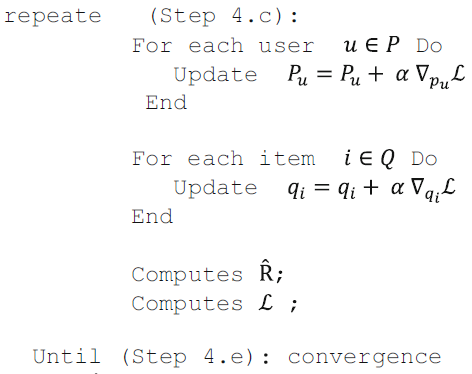
\includegraphics[width=7cm, height=6cm]{Latent-factor-Framework1.png}
		\end{figure}
		
	\end{enumerate}

	Koren et al. \cite{MFinRS} suggest that, though common in practices, stochastic gradient descent can be unfavorable compare to alternate least squares in two cases. The first case is when the system use parallelization for computing $q_i$ and $p_u$ independently with other item/user factors. The second case is when the system is centered on dense implicit data, which will turn looping as gradient descent does impractical.

	

	\subsection{Regularized SVD Model}

	\newcommand\myeq{\mathrel{\overset{\makebox[0pt]{\mbox{\normalfont\tiny\sffamily def}}}{=}}}
	\newcommand{\pluseq}{\mathrel{+}=}

	Regularized SVD model begins with Simon Funk in the Netflix challenge \cite{MFinRS}. This is essentially a ridge regularization and the main body of looping update part is
	\begin{equation}
		\begin{split}
			e_{ui}\ \myeq&\ r_{ui} - q_i^T p_u \\
			q_i\ \pluseq&\ \gamma (e_{ui} * p_u - \lambda * q_i) \\
			p_u\ \pluseq&\ \gamma (e_{ui} * q_i - \lambda * p_u)
		\end{split}
	\end{equation}

	The original purpose of regularization terms is to avoid overfitting and common approach includes lasso and ridge (or L1 L2) regularization \cite{RSVD-News}, as shown in Algorithm \ref{L1}.
	
	\floatname{algorithm}{Algorithm}
	\begin{algorithm}
		\caption{Update Main Body of SVD with Lasso (L1) Regularization\cite{RSVD-News}}
		\label{L1}
		\begin{algorithmic}
			\IF{$p_u \geq 0$}
				\STATE $p_u \pluseq \gamma (e_{ui} q_j - \lambda \alpha - \lambda p_u ( 1 - \alpha))$
			\ELSE
				\STATE $p_u \pluseq \gamma (e_{ui} q_j + \lambda \alpha - \lambda p_u ( 1 - \alpha))$
			\ENDIF
			
			\IF{$q_i \geq 0$}
				\STATE $q_i \pluseq \gamma (e_{ui} p_i - \lambda \alpha - \lambda q_i ( 1 - \alpha))$
			\ELSE
				\STATE $q_i \pluseq \gamma (e_{ui} p_i + \lambda \alpha - \lambda p_u ( 1 - \alpha))$			
			\ENDIF
		\end{algorithmic}
	\end{algorithm}

	An ALS implementation of SVD with ridge (L2) regularization is provided by Zheng et al. \cite{RSVD}.
	
	\renewcommand{\algorithmicrequire}{\textbf{Input:}}
	
	\begin{algorithm}
		\caption{ALS of SVD with Ridge (L2) Regularization\cite{RSVD}}
		\label{L1}
		\begin{algorithmic}
			\REQUIRE{rating matrix $R$, rank $k$, regularization weight $\lambda$}
			\STATE $L = \| R - P Q^T \|_F^2 + \lambda \| P \|_F^2 + \lambda \| Q \|_F^2$
			\STATE initialize $Q$ with some random values
			\REPEAT
				\STATE $ P = R Q(Q^TQ + \lambda I)^{-1} $
				\STATE $ Q = R^T P(P^T P + \lambda I)^{-1} $
			\UNTIL{$L$ converges} 
		\end{algorithmic}
	\end{algorithm}

	Zheng et al. \cite{RSVD} have proven that RSVD is still in SVD subspace and it converges generally faster than standard SVD approach. The RSVD objective function is not convex (RSVD is actually biconvex), but it still has a global optimal solution that can be obtained as the global optimal solution as a closed form \cite{RSVD}.
	
	Besides L1 and L2 regularization techniques, scholars also have interests on .
	
	% kernelized and weighted-lambda-regularization goes here



	\subsection{SVD++ Model}
	
	The traditional SVD method only considers users' explicit ratings but do not take implicit data into account. Although implicit data (mouse move, reading time, etc.) might not be publicly available, there is one kind of implicit data always available: whether a user rates on an item (rate vs. not rate). 
	
	
	SVD++ model was developed by Koren \cite{korenFactorization}. The complete formula is shown in equation \ref{SVD++}. 
	
	\begin{equation} \label{SVD++}
		\begin{split}
			\hat{r}_{ui} =& \ \mu + b_i + b_u \\ 
			& + q_i^T  (p_u + |N_u|^{-1/2} \sum_{j \in N_u}y_j) \\ 
			& + |R^k(i; u)|^{-1/2} \sum_{j \in R^k(i; u)} (r_{u_j} - b_{u_j}) w_{ij} + |N^k(i; u)|^{-1/2} \sum_{j \in N^k(i; u)} c_{ij}
		\end{split}
	\end{equation}
	
	
	Rule \ref{SVD++} is a 3-tier model. The first tier is $b_{ui}$ as mentioned before. 
	
	
	The second tier $q_i^T  (p_u + |N_{(u)}|^{-\frac{1}{2}} \sum_{j \in N_{(u)}}y_j)$ describes the intersection between user profile and item profile. We need to introduce a few notations to understand this tier:
	\begin{itemize}
		\item $R_u$ is the set of all items for which user $u$ provides a rating. $N_u$ is the set of all items for which user $u$ provides an implicit preference. $S^k(i)$ is the set of $k$ items rated by $u$ that are similar to item $i$.
		
		\item $N^k{(i; u)} = N_u \cap S^k (i)$. $R^k{(i; u)} = R_u \cap S^k (i)$
		
		\item $w_{ij}$ is a weight from item $j$ to $i$. $c_{ij}$ is a significance offset (indication of predictability by item $j$ to $i$)
	\end{itemize}
	
	The remaining terms form the final tier, or "neighborhood tier" called by Koren \cite{korenFactorization}, as it contributes some adjustments to the profile.
	
	The algorithm of SVD++ is shown in figure \ref{SVD++-Algo}.
	
	\begin{figure}[h]
		\centering
		\caption{SVD++ Algorithm}
		\label{SVD++-Algo}
		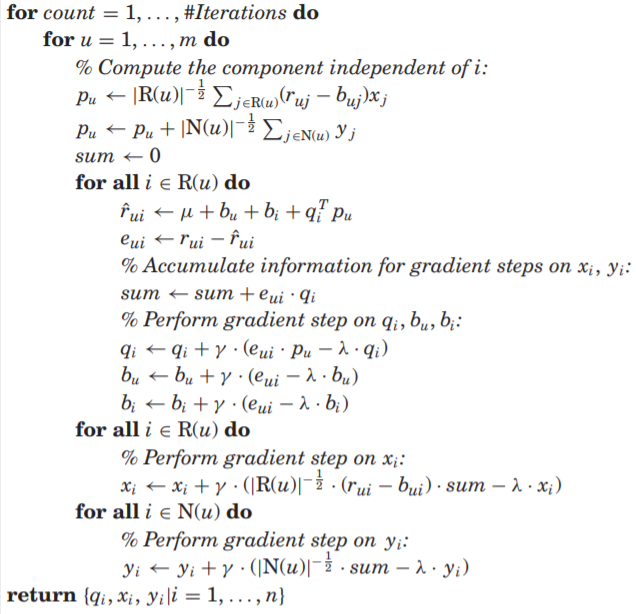
\includegraphics[width=9.5cm, height=9.5cm]{SVD++.png}
	\end{figure}
	
	The entire SVD++ model usually begins with standard SVD decomposition and calculation of similarity measure as mentioned before. After forming $S^k(i)$, a gradient descent algorithm will be applied to get predicted rating from equation \ref{SVD++}, as developed by Koren et al\cite{koren2010}.  
	
	SVD++ model arouses great research interests has been applied and tested in numerous dataset \cite{SVD++performance} \cite{korenFactorization} and it generally beats traditional SVD-CF model. However, the contribution of SVD++ is far more than an improvement in benchmark but a new field for exploration: context \cite{contextual}, or "any information that can be used to characterize the situation of entities" by Jallouli et al. Scholars then incorporate more contexts (trust, temporal dynamics, environmental information, etc.) into SVD++ method and developed methods like TrustMF, TimeSVD++, and more \cite{contextual} \cite{review}.
	
			
	Jallouli et al., for instance, suggests three modifications to SVD++ model to include influence of previously preferred items, user-user social information, and environmental information \cite{contextual}. The first modification brings the following rating prediction function (notice the term $\sum_{i \in I_u} y_i$ as latent factors of previously preferred items):
	
	\begin{equation}
		\hat{r}_{ui} = \mu + b_i + b_u  + (q_j^T + |I_u|^{-1/2}\sum_{i \in I_u} y_i) p_u
	\end{equation}
	
	The minimum objective function is presented as follows:
	
	\begin{equation}
		\begin{split}
			\mathcal{L} = &\ \dfrac{1}{2} \sum_{(u, j)} (\hat{r_{uj}} - r_{uj})^2 + \dfrac{\lambda}{2} \sum_{u \in U_j} |I_u|^{-1/2} b_u^2 + \dfrac{\lambda}{2} \sum_{j \in I_u} |U_j|^{-1/2} b_j^2 \\
			& + \dfrac{\lambda}{2} \sum_{u \in U_j} |I_u|^{-1/2} \|p_u\|_F^{2} + \dfrac{\lambda}{2} \sum_{j \in I_u} |U_j|^{-1/2} \|q_j\|_F^{2} \\
			& + \dfrac{\lambda}{2} \sum_{j \in I_u} |U_i|^{-1/2} \|y_i\|_F^{2}
		\end{split}
	\end{equation}
	
	The regularization term $|U_j|^{-1/2}$ and $|I_u|^{-1/2}$ are weighted-$\lambda$-regularization approach. We can then devise a gradient descent method for this minimum objective function. The second and third modification is essentially similar to the first one in structure and the formula is omitted here for brevity.
	
	% \section{Problems with Matrix Factorization Method}
	
	\subsection{Current Research Trends}
	\subsubsection{User Demographic Information}
	
	
	\subsubsection{Large-scale System Implementation}
	
	\section{Comparison and Discussion of SVD-Based Framework}



	\begin{table}
		\centering
		\begin{tabular}{|c|c|c|c|c|c|}
			\hline
			Technique & Explicit Rating & Implicit Rating & Data Imputation & Biases Used & Regularization \\ \hline
			SVD-CF & $\checkmark$ &  & $\checkmark$ &  &  \\ \hline
			RSVD-CF & $\checkmark$ &  & &  & $\checkmark$ \\ \hline
			SVD++ & $\checkmark$ & $\checkmark$ & & $\checkmark$ & $\checkmark$ \\ \hline
		\end{tabular}
		\caption{Comparison of SVD Based Techniques\cite{review}}
		\label{comparison}
	\end{table}
	
	
	\section{Experiment}
	% some data goes here	
	
	
	\section{Conclusion}

	\bibliographystyle{plain}
	\bibliography{reference.bib}
\end{document}